\documentclass[border=2pt]{standalone}
\usepackage{tikz}
\usepackage{lmodern}
\renewcommand{\familydefault}{\sfdefault}
\usetikzlibrary{calc}
% Data: canonical test split (n=1,949) and Stage-A binary gate (n=3,669)
\begin{document}
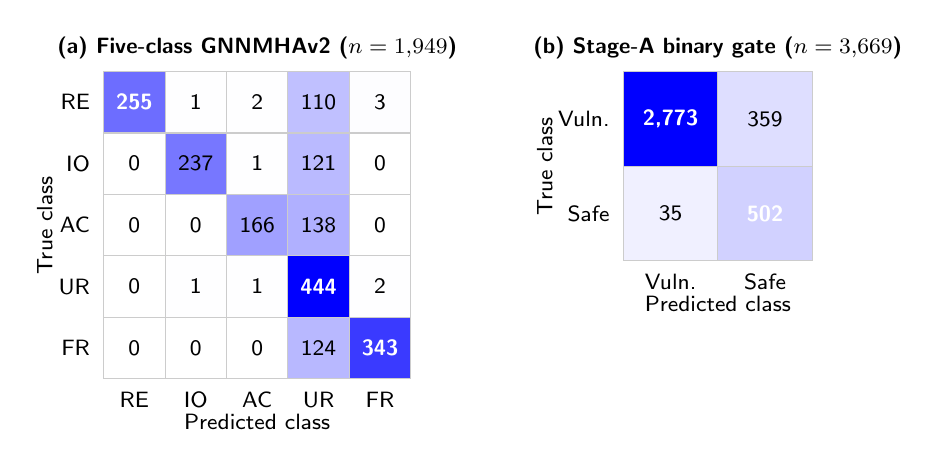
\begin{tikzpicture}[font=\footnotesize]
  \def\cs{0.78}
  % ---------------- (a) five-class ----------------
  \def\labels{{"RE","IO","AC","UR","FR"}}
  \foreach \r/\row in {0/{255,1,2,110,3},1/{0,237,1,121,0},2/{0,0,166,138,0},3/{0,1,1,444,2},4/{0,0,0,124,343}}{
    \foreach \v [count=\c from 0] in \row {
      \pgfmathsetmacro{\shade}{min(100,\v/444*100)}
      \pgfmathsetmacro{\txt}{\v>250 ? 1 : 0}
      \fill[blue!\shade!white] (\c*\cs,-\r*\cs) rectangle ++(\cs,-\cs);
      \draw[gray!40] (\c*\cs,-\r*\cs) rectangle ++(\cs,-\cs);
      \ifdim\txt pt>0.5pt
        \node[white,font=\footnotesize\bfseries] at (\c*\cs+\cs/2,-\r*\cs-\cs/2) {\v};
      \else
        \node[black] at (\c*\cs+\cs/2,-\r*\cs-\cs/2) {\v};
      \fi
    }
  }
  \foreach \n [count=\i from 0] in {RE,IO,AC,UR,FR}{
    \node[anchor=east] at (-0.05,-\i*\cs-\cs/2) {\n};
    \node[anchor=north] at (\i*\cs+\cs/2,-5*\cs-0.05) {\n};
  }
  \node[rotate=90] at (-0.75,-2.5*\cs) {True class};
  \node at (2.5*\cs,-5*\cs-0.55) {Predicted class};
  \node[font=\footnotesize\bfseries] at (2.5*\cs,0.3) {(a) Five-class GNNMHAv2 ($n=1{,}949$)};
  % ---------------- (b) binary gate ----------------
  \begin{scope}[xshift=6.6cm]
  \def\bs{1.2}
  \foreach \r/\row in {0/{2773,359},1/{35,502}}{
    \foreach \v [count=\c from 0] in \row {
      \pgfmathsetmacro{\shade}{min(100,\v/2773*100)}
      \pgfmathsetmacro{\shade}{max(\shade,6)}
      \fill[blue!\shade!white] (\c*\bs,-\r*\bs) rectangle ++(\bs,-\bs);
      \draw[gray!40] (\c*\bs,-\r*\bs) rectangle ++(\bs,-\bs);
    }
  }
  \node[white,font=\footnotesize\bfseries] at (0.5*\bs,-0.5*\bs) {2{,}773};
  \node at (1.5*\bs,-0.5*\bs) {359};
  \node at (0.5*\bs,-1.5*\bs) {35};
  \node[white,font=\footnotesize\bfseries] at (1.5*\bs,-1.5*\bs) {502};
  \node[anchor=east] at (-0.05,-0.5*\bs) {Vuln.};
  \node[anchor=east] at (-0.05,-1.5*\bs) {Safe};
  \node[anchor=north] at (0.5*\bs,-2*\bs-0.05) {Vuln.};
  \node[anchor=north] at (1.5*\bs,-2*\bs-0.05) {Safe};
  \node at (\bs,-2*\bs-0.55) {Predicted class};
  \node[rotate=90] at (-1.0,-\bs) {True class};
  \node[font=\footnotesize\bfseries,align=center] at (\bs,0.3) {(b) Stage-A binary gate ($n=3{,}669$)};
  \end{scope}
\end{tikzpicture}
\end{document}
